\begin{center}
\LARGE
Delprøve uden hjælpemidler 
\end{center}
\stepcounter{section}

\begin{opgavetekst}{Opgave 1}
\end{opgavetekst}
	\begin{delopgave}{}{1}
		Reducér udtrykket 
		\begin{align*}
			 \frac{(a^3+b)ab^2-a^4b^2}{b^2}.
		\end{align*}
	\end{delopgave}
%%%%%%%%%%%%%%%%%%%%%%%%%%%%%%%%%%%%%%%%%%%%%%%%%%%%%%%%%%%%%%%%%%%%%%%
%							Ny Opgave!!!!!							%
%%%%%%%%%%%%%%%%%%%%%%%%%%%%%%%%%%%%%%%%%%%%%%%%%%%%%%%%%%%%%%%%%%%%%%%
\begin{opgavetekst}{Opgave 2}
	En funktion $f:\mathbb{R}^2 \to \mathbb{R}$ er givet ved
	\begin{align*}
		f(x,y) = x^2-2y^2+4x-8y-16.
	\end{align*}
\end{opgavetekst}
	\begin{delopgave}{}{1}
		Bestem $f(2,-3)$.
	\end{delopgave}
	\begin{delopgave}{}{2}
		Bestem det stationære punkt for $f$. 
	\end{delopgave}
	\begin{delopgave}{}{3}
		Bestem arten af det stationære punkt. 
	\end{delopgave}
%%%%%%%%%%%%%%%%%%%%%%%%%%%%%%%%%%%%%%%%%%%%%%%%%%%%%%%%%%%%%%%%%%%%%%%
%							Ny Opgave!!!!!							%
%%%%%%%%%%%%%%%%%%%%%%%%%%%%%%%%%%%%%%%%%%%%%%%%%%%%%%%%%%%%%%%%%%%%%%%
\begin{opgavetekst}{Opgave 3}
	En linje $l$ er givet ved
	\begin{align*}
		l: \ 3x -4y + 6 = 0,
	\end{align*}
	og et punkt $P$ er givet ved $P(2,-2)$.
\end{opgavetekst}
\begin{delopgave}{}{1}
	Bestem den korteste afstand fra $l$ til $P$. 
\end{delopgave}
%%%%%%%%%%%%%%%%%%%%%%%%%%%%%%%%%%%%%%%%%%%%%%%%%%%%%%%%%%%%%%%%%%%%%%%
%							Ny Opgave!!!!!							%
%%%%%%%%%%%%%%%%%%%%%%%%%%%%%%%%%%%%%%%%%%%%%%%%%%%%%%%%%%%%%%%%%%%%%%%
\begin{opgavetekst}{Opgave 4}
\end{opgavetekst}
\begin{delopgave}{}{1}
	Differentier følgende funktion.
	\begin{align*}
		\sqrt{x}\cdot e^{2x}.
	\end{align*}
\end{delopgave}
\begin{delopgave}{}{2}
	Differentier følgende funktion.
	\begin{align*}
		 e^{x^3-2x^2-1}.
	\end{align*}
\end{delopgave}
%%%%%%%%%%%%%%%%%%%%%%%%%%%%%%%%%%%%%%%%%%%%%%%%%%%%%%%%%%%%%%%%%%%%%%%
%							Ny Opgave!!!!!							%
%%%%%%%%%%%%%%%%%%%%%%%%%%%%%%%%%%%%%%%%%%%%%%%%%%%%%%%%%%%%%%%%%%%%%%%
\begin{opgavetekst}{Opgave 6}
	En differentialligning er givet ved
	\begin{align}\label{eq:ligning1}
		\frac{dy}{dx} = 7x^2y.
	\end{align}
\end{opgavetekst}
\begin{delopgave}{}{1}
	Vis, at funktionen $f:\mathbb{R} \to \mathbb{R}$ givet ved
	\begin{align*}
		f(x) = e^{\frac{7}{3}x^3}.
	\end{align*}
	er en partikulær løsning til \eqref{eq:ligning1}.
\end{delopgave}
%%%%%%%%%%%%%%%%%%%%%%%%%%%%%%%%%%%%%%%%%%%%%%%%%%%%%%%%%%%%%%%%%%%%%%%
%							Ny Opgave!!!!!							%
%%%%%%%%%%%%%%%%%%%%%%%%%%%%%%%%%%%%%%%%%%%%%%%%%%%%%%%%%%%%%%%%%%%%%%%
\begin{opgavetekst}{Opgave 7}
\end{opgavetekst}
\begin{delopgave}{}{1}
	Udregn følgende ubestemte integral
	\begin{align*}
		\int e^{7\sin(x)+3\cos(x)}(7\cos(x)-3\sin(x))dx.
	\end{align*}
\end{delopgave}
%%%%%%%%%%%%%%%%%%%%%%%%%%%%%%%%%%%%%%%%%%%%%%%%%%%%%%%%%%%%%%%%%%%%%%%
%							Ny Opgave!!!!!							%
%%%%%%%%%%%%%%%%%%%%%%%%%%%%%%%%%%%%%%%%%%%%%%%%%%%%%%%%%%%%%%%%%%%%%%%
\begin{opgavetekst}{Opgave 8}
	En differentialligning er givet ved
	\begin{align}\label{eq:ligning2}
		y' = 10y.
	\end{align}
\end{opgavetekst}
\begin{delopgave}{}{1}
	Bestem en partikulær løsning til \eqref{eq:ligning2}, der går gennem punktet $(0,4)$. 
\end{delopgave}

\newpage
\begin{center}
\LARGE
Delprøve med hjælpemidler 
\end{center}
\stepcounter{section}
%%%%%%%%%%%%%%%%%%%%%%%%%%%%%%%%%%%%%%%%%%%%%%%%%%%%%%%%%%%%%%%%%%%%%%%
%							Ny Opgave!!!!!							%
%%%%%%%%%%%%%%%%%%%%%%%%%%%%%%%%%%%%%%%%%%%%%%%%%%%%%%%%%%%%%%%%%%%%%%%
\begin{opgavetekst}{Opgave 9}
	\begin{center}
		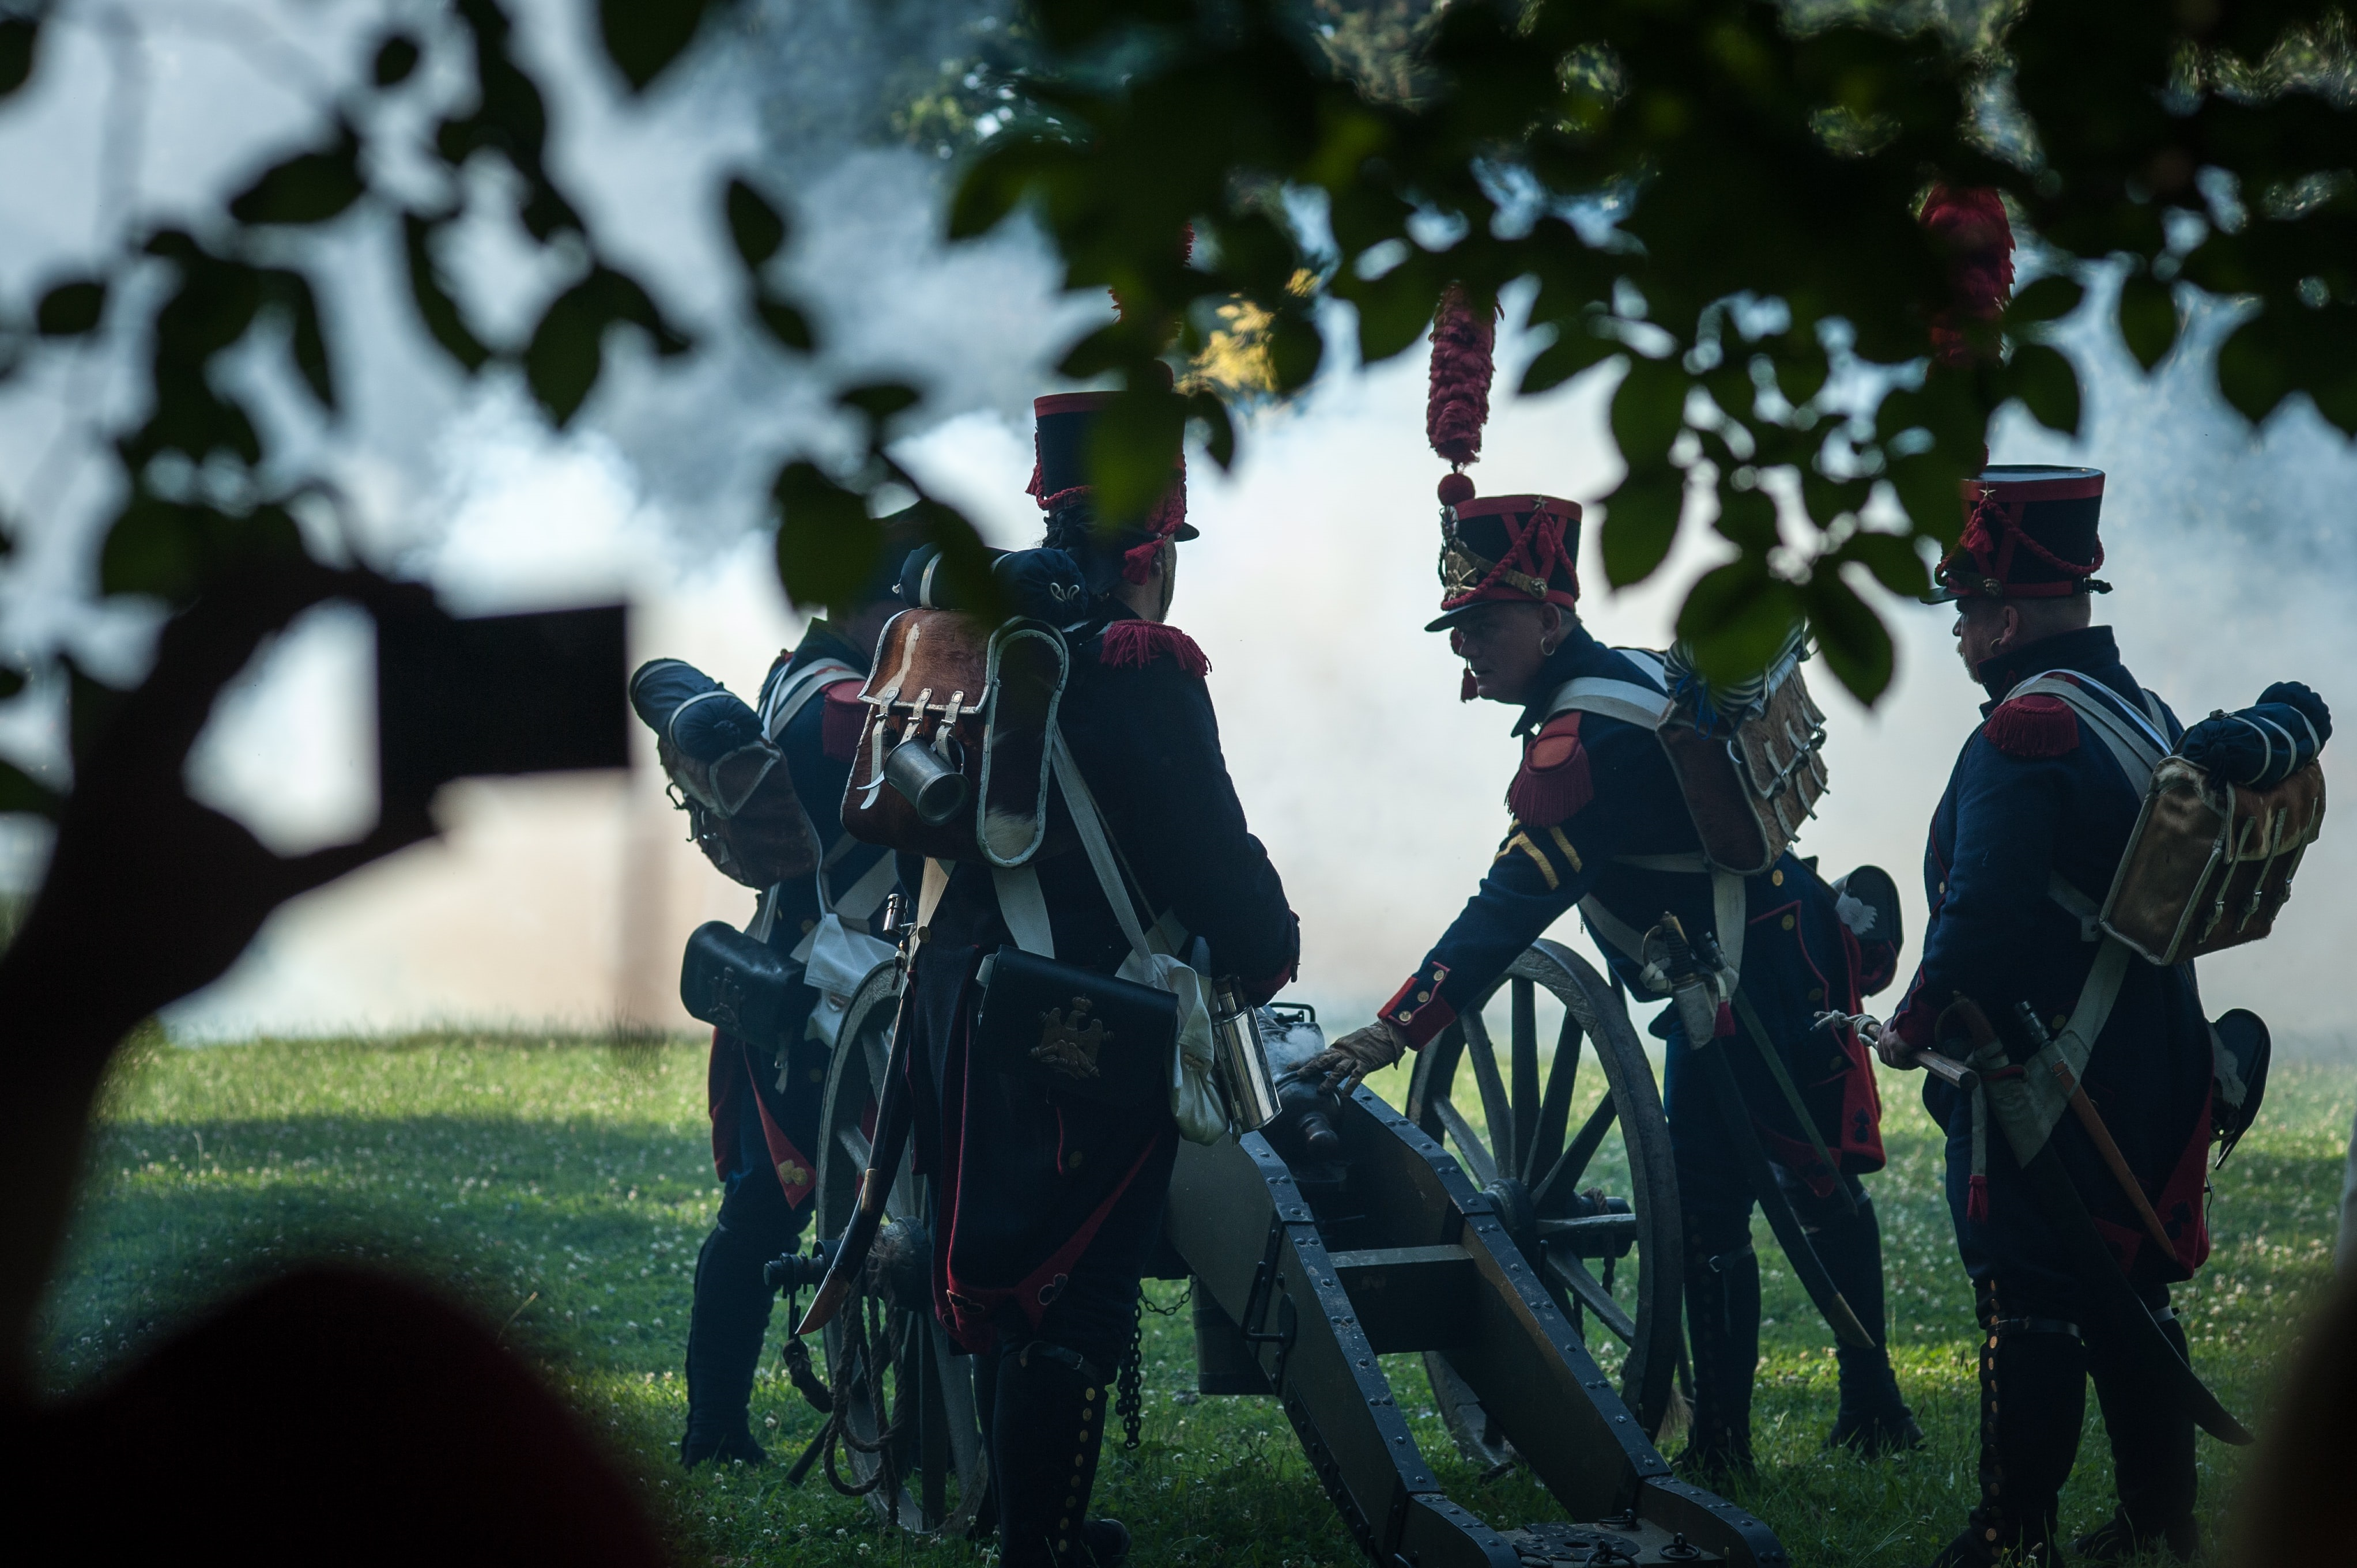
\includegraphics[width=0.6\textwidth]{Billeder/kanon.jpg}
	\end{center}
	Under den 2. Slesviske krig skulle de østrigske og preussiske kanoner skyde over Vemmingbund for at ramme de danske skanser ved Dybbøl mølle. Skudafstanden afhænger af affyringsvinklen på kanonen
	og for at skyde den rigtige afstand er det vigtigt at kende den korrekte affyringsvinkel. Af Tab.  \ref{tab:kanon} kan sammenhængen mellem affyringsvinklen $x$ (i grader) og skudafstanden $D$
	(i meter) ses.
	\begin{table}[H]
		\centering
		\begin{tabular}{c|c|c|c|c|c|c|c}
		$x$ &10 & 20 & 30 & 40 & 50 & 60 & 70 \\
		\hline
		$D$ & 1197 & 2089 & 2655 & 2968 & 3022 & 2659 & 2082
		\end{tabular}
		\caption{Sammenhæng mellem skudafstand (i meter) og affyringsvinkel (i grader)}
		\label{tab:kanon}
	\end{table}\phantom{h}
	En model for affyringsafstanden $D$ som funktion af affyringsvinklen $x$ er givet ved
	\begin{align*}
		D(x) = ax^2+bx+c
	\end{align*}
\end{opgavetekst}
\begin{delopgave}{}{1}
	Brug tallende fra Tab. \ref{tab:kanon} til at bestemme en forskrift for $D$.
\end{delopgave}
\begin{meretekst}
	Det oplyses, at der er $1.8$km fra de preussisk/østrigske skanser til Skanse 1 ved Vemmingbund. 
\end{meretekst}
\begin{delopgave}{}{2}
	Hvilken affyringsvinkel skal bruges for at ramme Skanse 1?
\end{delopgave}
\begin{delopgave}{}{3}
	Hvad er ifølge modellen den maksimale skudafstand?
\end{delopgave}
%%%%%%%%%%%%%%%%%%%%%%%%%%%%%%%%%%%%%%%%%%%%%%%%%%%%%%%%%%%%%%%%%%%%%%%
%							Ny Opgave!!!!!							%
%%%%%%%%%%%%%%%%%%%%%%%%%%%%%%%%%%%%%%%%%%%%%%%%%%%%%%%%%%%%%%%%%%%%%%%
\begin{opgavetekst}{Opgave 10}
	\begin{center}
		
\includegraphics[width=0.6\textwidth]{Billeder/medicin.jpg}
	\end{center}
	For et bestemt lægemiddel har man målt nedbrydningshastigheden $y'$ (i mg/l per time ) i kroppen som funktion af koncentrationen $y$ (i mg/l) af lægemiddelet. Disse tal kan ses af Tab.
	\ref{tab:medicin}.
	\begin{table}[H]
	\centering
	\begin{tabular}{c|c|c|c|c|c|c|c}
		$y$ (i mg/l) & -998.6 & -835.7 & -670.6 & -505.4 & -340.7 & -175.6 & -9.5\\
		\hline
		$y'$ (i mg/l/t) & 52.2 & 44.5 & 38.1 & 29.2 & 23.9 & 19.7 & 10.9
	\end{tabular}
	\caption{Nedbrydningshastighed af lægemiddel som funktion af koncentration.}
	\label{tab:medicin}
	\end{table}
	Det antages, at sammenhængen mellem $y$ og $y'$ er på formen
	\begin{align}\label{eq:difflign3}
		y' = b-ay.
	\end{align}
\end{opgavetekst}
\begin{delopgave}{}{1}
	Brug datasættet til at bestemme $a$ og $b$.
\end{delopgave}
\begin{delopgave}{}{2}
	Udnyt, at begyndelseskoncentrationen af lægemiddelet var 1000 mg/l til at bestemme en partikulær løsning til differentialligningen \eqref{eq:difflign3}. 
\end{delopgave}
\begin{delopgave}{}{3}
	Afgør, hvornår koncentrationen af lægemiddelet er på 2 mg/l.
\end{delopgave}
%%%%%%%%%%%%%%%%%%%%%%%%%%%%%%%%%%%%%%%%%%%%%%%%%%%%%%%%%%%%%%%%%%%%%%%
%							Ny Opgave!!!!!							%
%%%%%%%%%%%%%%%%%%%%%%%%%%%%%%%%%%%%%%%%%%%%%%%%%%%%%%%%%%%%%%%%%%%%%%%
\begin{opgavetekst}{Opgave 11}
	En cirkel $C$ er givet ved ligningen 
	\begin{align*}
		C: \ x^2-6x+y^2-10y=30
	\end{align*}
\end{opgavetekst}
\begin{delopgave}{}{1}
	Bestem centrum og radius for $C$.
\end{delopgave}
\begin{meretekst}
	En linje $l$ er givet ved ligningen 
	\begin{align*}
		l: \ y = -2x+5.
	\end{align*}
\end{meretekst}
\begin{delopgave}{}{2}
	Bestem skæringspunkterne $P$ og $Q$ mellem $l$ og $C$. 
\end{delopgave}
\begin{delopgave}{}{3}
	Bestem en ligning for tangenten til cirklen i både $P$ og $Q$.
\end{delopgave}
%%%%%%%%%%%%%%%%%%%%%%%%%%%%%%%%%%%%%%%%%%%%%%%%%%%%%%%%%%%%%%%%%%%%%%%
%							Ny Opgave!!!!!							%
%%%%%%%%%%%%%%%%%%%%%%%%%%%%%%%%%%%%%%%%%%%%%%%%%%%%%%%%%%%%%%%%%%%%%%%
\begin{opgavetekst}{Opgave 12}
	En funktion $f: \mathbb{R} \to \mathbb{R}$ er givet ved
	\begin{align*}
		f(x) = x^3+7x^2-15.
	\end{align*}	 
\end{opgavetekst}
\begin{delopgave}{}{1}
	Tegn $f$ på intervallet $[-8,4]$.
\end{delopgave}
\begin{delopgave}{}{2}
	Bestem rødderne for $f$. 
\end{delopgave}
\begin{meretekst}
	Grafen for $f$ afgrænser sammen med $x$-aksen området $A_1$, der ligger over $x$-aksen og området $A_2$, der ligger under $x$-aksen.
\end{meretekst}
\begin{delopgave}{}{3}
	Bestem det samlede areal af $A_1$ og $A_2$. 
\end{delopgave}